%% AllSERP — ACM SIGIR / CHIIR submission target.
%% Build: ./build.sh --acmart  (or directly: latexmk -xelatex paper.tex)

\documentclass[sigconf,authorversion,natbib=true]{acmart}

%% Override copyright/conference for working draft; replace at venue submission.
\setcopyright{cc}
\setcctype{by}
\copyrightyear{2026}
\acmYear{2026}
\acmConference[arXiv preprint]{}{2026}{}

%% Strip ACM Reference Format / DOI / ISBN until accepted
\settopmatter{printacmref=false}
\acmDOI{}
\acmISBN{}
\renewcommand\footnotetextcopyrightpermission[1]{}

\usepackage{xurl}
\usepackage{booktabs}

\begin{document}

\title{AllSERP: Exhaustive Per-Element Enrichment of the Versatile AdSERP Dataset}

\author{Andy Edmonds}
\email{andyed@gmail.com}
\affiliation{%
  \institution{Independent}
  \city{}
  \country{}
}

\renewcommand{\shortauthors}{Edmonds}

\begin{abstract}
We release \textbf{AllSERP}, a typed AOI and per-element behavioral enrichment of the AdSERP commercial-intent SERP corpus~\cite{latifzadeh2025adserp}. AdSERP ships 2,776 trials of full-page screenshots, captured SERP HTML, 150~Hz Gazepoint eye tracking, \texttt{evtrack} mouse telemetry~\cite{leiva2013evtrack}, scroll, and pupil signals against real Google SERPs collected before AI Overviews, but its bounding boxes cover only ad surfaces (15.5\,\% of attributable clicks). AllSERP adds pixel-accurate organic and widget bboxes via screenshot-anchored CV, semantic types across thirteen element types via an HTML parser, an inter-result gap-fill flavor (\texttt{typed\_gapfill}), and X+Y click attribution that reaches 91.7\,\% of the corpus while flagging the rest at trial level. The typed ad-vs-non-ad partition is internally consistent with the shipped ad rectangles (0 disagreements across 38,250 classifications). We ship the pipeline, per-trial JSONs, a corpus CSV, and a browser-based replay viewer. Everything is reproducible from the AdSERP Zenodo volume. The release enables per-element click, fixation, regression, and above-fold analyses that the shipped ads-vs-organic split could not resolve.
\end{abstract}

\begin{CCSXML}
<ccs2012>
   <concept>
       <concept_id>10002951.10003317.10003331</concept_id>
       <concept_desc>Information systems~Users and interactive retrieval</concept_desc>
       <concept_significance>500</concept_significance>
       </concept>
   <concept>
       <concept_id>10002951.10003317.10003359</concept_id>
       <concept_desc>Information systems~Web log analysis</concept_desc>
       <concept_significance>300</concept_significance>
       </concept>
   <concept>
       <concept_id>10003120.10003123.10010860</concept_id>
       <concept_desc>Human-centered computing~User studies</concept_desc>
       <concept_significance>300</concept_significance>
       </concept>
 </ccs2012>
\end{CCSXML}

\ccsdesc[500]{Information systems~Users and interactive retrieval}
\ccsdesc[300]{Information systems~Web log analysis}
\ccsdesc[300]{Human-centered computing~User studies}

\keywords{search engine results pages, multimodal datasets, eye tracking, mouse cursor tracking, area of interest, dataset enrichment}

\maketitle

\section{Introduction}\label{sec:intro}

AdSERP~\cite{latifzadeh2025adserp} is the only public IR dataset that combines eye gaze, cursor, scroll, pupil, and click telemetry against ground-truth screenshots and captured SERP HTML on commercial-intent Google SERPs at thousands-of-trials scale. Two early uses prove what the substrate carries. AdSight~\cite{villaizan2025adsight} predicts per-slot fixation time at NDCG = 96.07~$\pm$~0.04 from cursor trajectories conditioned on slot metadata (slot type, normalized center position). Pupil-cognitive-load methods are being developed against AdSERP gaze on this corpus: real-time LF/HF~\cite{duchowski2026rtlfhf} and per-fixation arousal via RIPA2~\cite{jayawardena2025ripa2}. AllSERP raises the resolution at which work like these can run by replacing AdSight's four-slot taxonomy with nine main-axis element types and by typing every main-axis card the user sees.

The shipped ad rectangles cover only ad surfaces: roughly \textbf{15.5\,\% of attributable clicks}. The remaining $\sim$84.5\,\% land on organics, knowledge panels, image packs, People-Also-Ask widgets, and other untyped surfaces. Per-rank claims on AdSERP that pool ads with organics under ``absolute rank,'' or estimate organic geometry from h3 heading counts (which assume uniform result heights, though actual layouts vary by 80--320~px), have inherited that gap. AllSERP closes it.

\paragraph{Anticipated user community} Click-model researchers (cascade / DCM / UBM lineage and successors), attention and cognitive-load groups using AdSERP for pupil-method development, AdSight-style cursor-attention modelers, and IR replication researchers comparing pre-AI-Overviews behavior against post-rollout SERPs.

\paragraph{Contributions}\hfill
\begin{enumerate}
  \item \textbf{Screenshot-anchored typed AOI extraction} with per-trial JSON output covering organic, dd\_top, native\_ad, dd\_right, top\_places, knowledge\_panel, paa, image\_pack, related\_searches, pagination, other\_widget, unknown\_widget, and chrome surfaces.
  \item \textbf{Inter-result gap-fill and X+Y bbox-aware click attribution.} The gap-fill flavor extends adjacent organic bboxes via midpoint-split and uses X+Y containment, with a trial-level filter flagging off-axis clicks (right-rail ads, page chrome, far-off-target).
  \item \textbf{Internal-consistency validation} against shipped ground truth: 38,250 ad-classification comparisons, 0 disagreements. Structural rather than independent-annotator (\S\ref{sec:validation}).
  \item \textbf{Descriptive observed-behavior inventory} for nine main-axis element types: click share, fixation coverage, regression rate, above-fold incidence, on the full 2,776-trial corpus.
  \item \textbf{Public release.} Single-script pipeline, per-trial JSONs, corpus CSV, and a browser-based replay viewer (\S\ref{sec:release}). MIT code, CC-BY-4.0 derived data, matching the AdSERP corpus license.
\end{enumerate}

\section{Pipeline}\label{sec:pipeline}

\begin{figure*}[t]
  \centering
  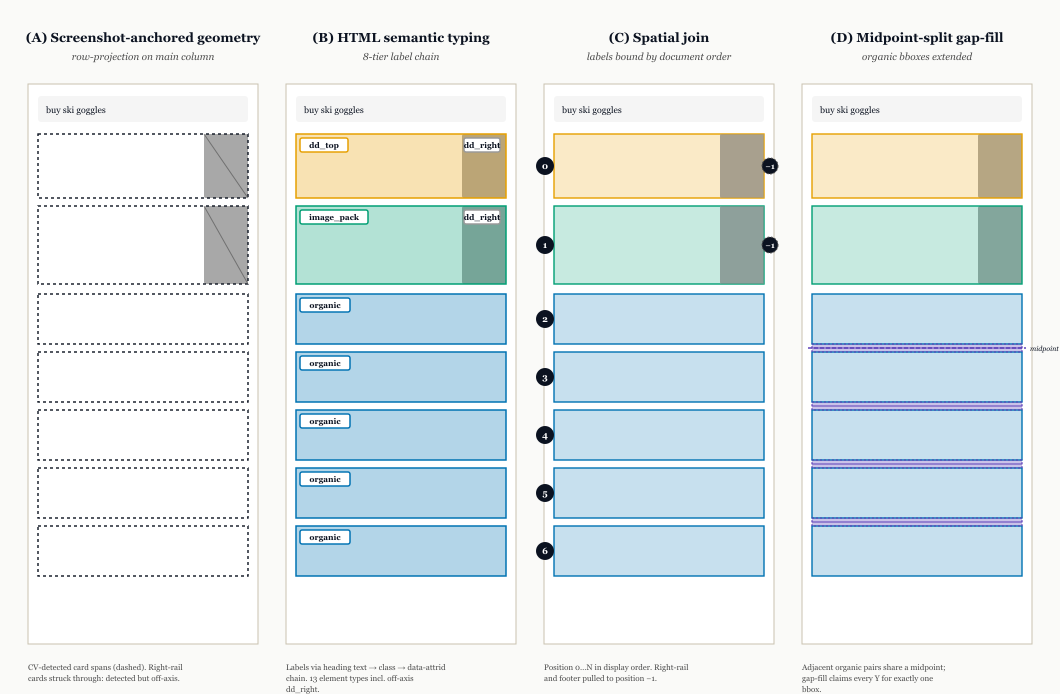
\includegraphics[width=\textwidth]{figs/fig_pipeline.png}
  \Description[Four-panel pipeline diagram on a synthetic SERP]{Four panels show the same synthetic Google SERP with progressive overlays: Phase A draws dashed brackets around CV-detected card spans; Phase B colours each card with its element type and adds a labelled chip; Phase C numbers each main-axis card 0 through 6 in display order with right-rail cards marked as off-axis; Phase D adds purple shaded gap-fill regions between adjacent organic results, with a midpoint annotation marking the boundary.}
  \caption{The four-phase pipeline applied to a synthetic SERP. \textbf{(A)} CV row-projection on the main column produces card spans (dashed outlines). Right-rail dd\_right cards are detected but routed off-axis. \textbf{(B)} Each main-axis card receives a label from an 8-tier HTML chain. \textbf{(C)} Labels are bound to geometry by document order. Each main-axis card receives a position 0\dots N; right-rail and footer cards get position $-1$. \textbf{(D)} Adjacent organic pairs share a midpoint. The upper bbox extends down and the lower extends up, so every Y in the column belongs to one bbox. dd\_top and image\_pack are unchanged.}
  \label{fig:pipeline}
\end{figure*}

\subsection{Why screenshot-anchored}

The AdSERP team's published methodology extracted AOIs from the DOM at collection time~\cite{latifzadeh2025adserp}, the cleanest source when the page is live. For \emph{downstream reuse}, that route fails: re-rendering the saved 2022--2023 HTML in a 2026 browser produces 13--45~px layout drift relative to the original screenshots, well within three years of separation. Drift sources include missing external assets, Chrome version differences, font drift, and Google's continual A/B-testing of SERP rendering. The shipped fixation and cursor streams are pixel-coordinated against the screenshots, so AllSERP anchors AOI geometry to those screenshots via CV and uses HTML only for structural labels. This complements the AdSERP team's collection-time DOM approach: the DOM is cleanest at capture, and the screenshots are what survive for downstream reuse.

\subsection{Four phases}

Phase~A produces card spans by per-row standard-deviation row-projection on the main column, with shipped ad rectangles taking precedence on overlap and a composite-trigger height triggering inner subdivision for image\_pack / paa / top\_stories. Phase~B walks the saved HTML and assigns each card a type label via an 8-tier priority chain (heading text $\rightarrow$ structural class signatures $\rightarrow$ \texttt{data-attrid} $\rightarrow$ fallback structural patterns), producing 13 etypes including a \texttt{chrome} sweep for footer artifacts. Phase~C binds labels to geometry by document order, the only stable axis when HTML and screenshot don't share a coordinate space. Phase~D adds the \texttt{typed\_gapfill} flavor by extending each pair of adjacent organic bboxes to their shared midpoint, clamped so an organic never crosses an ad or widget. Both flavors are released: the \textbf{tight-bbox flavor} (\texttt{typed}, Phase A $\rightarrow$ C) and the \textbf{gap-fill flavor} (\texttt{typed\_gapfill}, Phase A $\rightarrow$ D). Analyses can pick the attribution semantics that match their use. Source code, parameter values, and per-trial outputs ship in the upstream repository (\S\ref{sec:release}).

\subsection{Click attribution and trial filter}

Click attribution under the gap-fill flavor requires X \emph{and} Y containment in a main-axis AOI bbox, with a small $\pm 5$~X / $\pm 10$~Y tolerance fallback for link-padding clicks. Y-only attribution would route right-rail ads, page chrome, and far-off-target clicks into adjacent main-axis AOIs that share their Y. X containment refuses those. The \texttt{is\_main\_axis\_click(trial\_id)} helper returns True iff a trial's final click lands in a main-axis AOI under this rule. In the AdSERP corpus, 231 trials are flagged at trial level: 67 dd\_right (right-rail ad clicks), 91 page-chrome / search-tools / far-off-target, 73 with no clicks recorded or pathological click coordinates. Producers computing click-outcome features drop these trials.

\section{Validation}\label{sec:validation}

The shipped ad rectangles~\cite{latifzadeh2025adserp} were extracted by the AdSERP authors against the same screenshots the gaze and cursor streams were recorded against, so they are pixel-anchored to the same truth source as our extraction. Phase~C ad propagation matches the shipped rectangles across all three ad etypes (\texttt{dd\_top}, \texttt{native\_ad}, \texttt{dd\_right}) with \textbf{0 disagreements across 38,250 individual classifications}, mean IoU = 1.000, and 0 of 26,590 Phase~A \texttt{organic\_result} bboxes overlapping any shipped ad rectangle. We frame this as an \textbf{internal-consistency check} rather than independent-annotator validation: Phase~C inherits ad identity by spatial overlap and is then checked against the same rectangles. The deeper non-ad partition (organic vs paa vs image\_pack vs the rest) lacks an external label set. We validate it against the HTML structure that Phase~B's chain consumes and against visual spot-check on the curated 147-trial replay set. Independent-annotator validation on a held-out subset is named as future work.

\paragraph{Gaze-cursor spatial registration} Beyond the ad-rectangle internal-consistency check, the resource depends on gaze and cursor streams sharing a coordinate space. We probe this end-to-end: in the lead-up to the final click, did gaze ever land near the click target? For each trial with a final click ($n = 2{,}752$ with at least one fixation in the lead window), we take all gaze fixations whose midpoint falls in $[t_{\textit{click}} - 1500$\,ms, $t_{\textit{click}}]$ and compute the minimum Euclidean distance from any such fixation to the click coordinates. Median: \textbf{128.8\,px}. Interquartile range: 80.4--206.5\,px. p95: 446.2\,px. Trials with a minimum gap exceeding 250\,px ($\sim$$3^\circ$ visual angle, past the GP3~HD calibration tolerance): \textbf{17.8\,\% (489)}. The concurrent at-click distance (the distance from the fixation that encompasses $t_{\textit{click}}$ to the click itself) is intentionally not the right metric here: gaze leads cursor by several hundred milliseconds on SERPs, so by $t_{\textit{click}}$ gaze has typically moved on, and the concurrent median is 506.8\,px. The lead-window minimum is the spatial-registration probe. The concurrent median is reported only to disambiguate the two questions. Producer: \path{scripts/audit_gaze_cursor_coverage.py}. Full per-trial output and provenance metadata: \path{scripts/output/allserp/gaze_cursor_coverage.json}.

\begin{figure}[t]
  \centering
  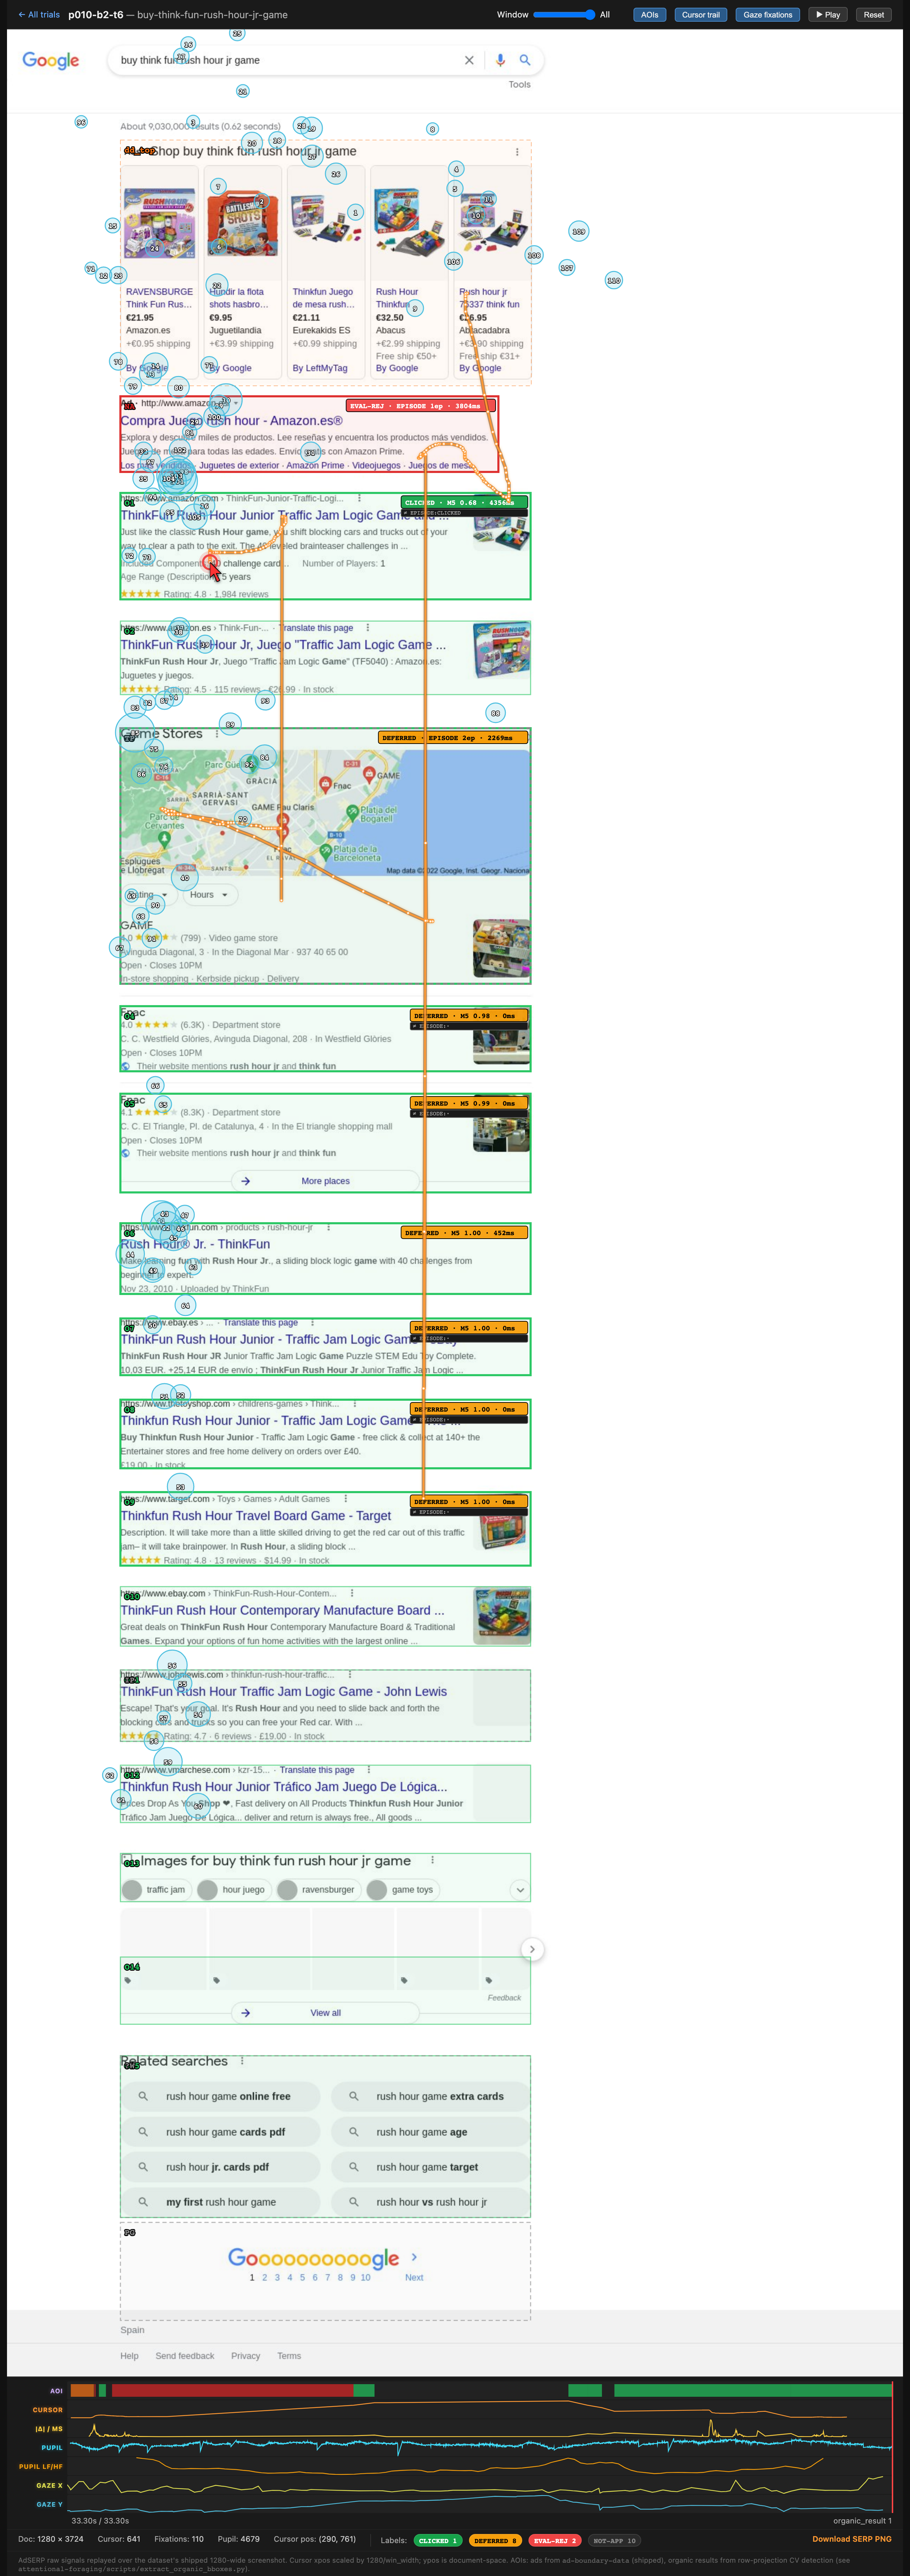
\includegraphics[width=\columnwidth,height=0.42\textheight,keepaspectratio]{figs/fig4_replay_p010-b2-t6.png}
  \Description[Replay viewer screenshot of one AdSERP trial]{Portrait screenshot of the AllSERP replay viewer: a Google SERP with coloured AOI rectangles, gaze fixation circles, an orange cursor trajectory, and seven sparkline tracks at the bottom (cursor speed, XY delta, pupil, LF/HF, gaze X, gaze Y, AOI presence).}
  \caption{Replay viewer rendering of trial p010-b2-t6 (viewer ships with the repo, \S\ref{sec:release}). Coloured rectangles: typed AOIs. Numbered circles: gaze fixations sized by dwell. Orange polyline: cursor trajectory. Sparklines: cursor speed, XY delta, pupil, LF/HF, gaze X/Y, AOI presence.}
  \label{fig:replay}
\end{figure}

\section{Element-Type Inventory}\label{sec:inventory}

Population: 2,775 trials processed (1 trial dropped for missing meta or fixations), yielding 37,142 typed AOI rows under the gap-fill flavor. Table~\ref{tab:inventory} reports the per-element-type behavioral inventory. Column denominators differ across columns (see notes below).

\begin{table*}[t]
  \caption{Per-element-type behavioral inventory under the gap-fill flavor. Etypes ordered by AOI count, descending.}
  \label{tab:inventory}
  \small
  \begin{tabular}{lrrrrrr}
    \toprule
    etype & n\_aois & fixated \% & n\_clicks & click \% & regressive \% & above-fold \% \\
    \midrule
    organic         & 22,346 & 55.6           & 2,084 & 79.1 & 57.8 & 97.3 \\
    native\_ad      & 9,214  & 36.4           & 156   & 5.9  & 46.9 & 37.8 \\
    image\_pack     & 1,584  & 52.0           & 55    & 2.1  & 59.3 & 20.5 \\
    dd\_top         & 1,582  & \textbf{99.7}  & 254   & 9.6  & 83.4 & 57.0 \\
    unknown\_widget & 788    & 17.4           & 7     & 0.3  & 26.3 & 0.0  \\
    paa             & 769    & 40.6           & 44    & 1.7  & 45.8 & 11.3 \\
    knowledge\_panel& 745    & 48.6           & 31    & 1.2  & 44.5 & 3.5  \\
    top\_places     & 84     & 54.8           & 1     & 0.0  & 50.0 & 2.1  \\
    other\_widget   & 50     & 58.0           & 2     & 0.1  & 44.8 & 1.1  \\
    \bottomrule
  \end{tabular}
\end{table*}

\paragraph{Column notes} \emph{Fixated~\%} is over the etype's full AOI population. \emph{Click~\%} is over 2,634 click events attributed to a gap-fill AOI (89\,\% of all click events). The remaining 11\,\% are intermediate cursor clicks that landed off any main-axis AOI. The 91.7\,\% corpus-level rate quoted in the abstract counts trials whose \emph{final} click lands main-axis under the trial filter, a different denominator. \emph{Regressive~\%} is over the fixated subset and is therefore not directly comparable across etypes whose fixation rates differ widely (organic 56\,\%, dd\_top 99.7\,\%). \emph{Above-fold~\%} is the share of the 2,776 trials in which at least one AOI of that etype sits in the initial viewport.

\paragraph{Read} dd\_top reaches near-universal fixation but only 9.6\,\% of clicks. The click-fixation dissociation is preserved at element-type granularity, sharper than at the ad-vs-organic level the original AdSERP analysis used. The pattern (36.4\,\% vs 5.9\,\% for native\_ad, 99.7\,\% vs 9.6\,\% for dd\_top) matches an attention-without-commitment account. Organic results occupy the initial viewport on 97\,\% of trials and capture 79\,\% of clicks. Widgets and ads dominate above-fold geometry but not click outcomes.

\begin{figure*}[t]
  \centering
  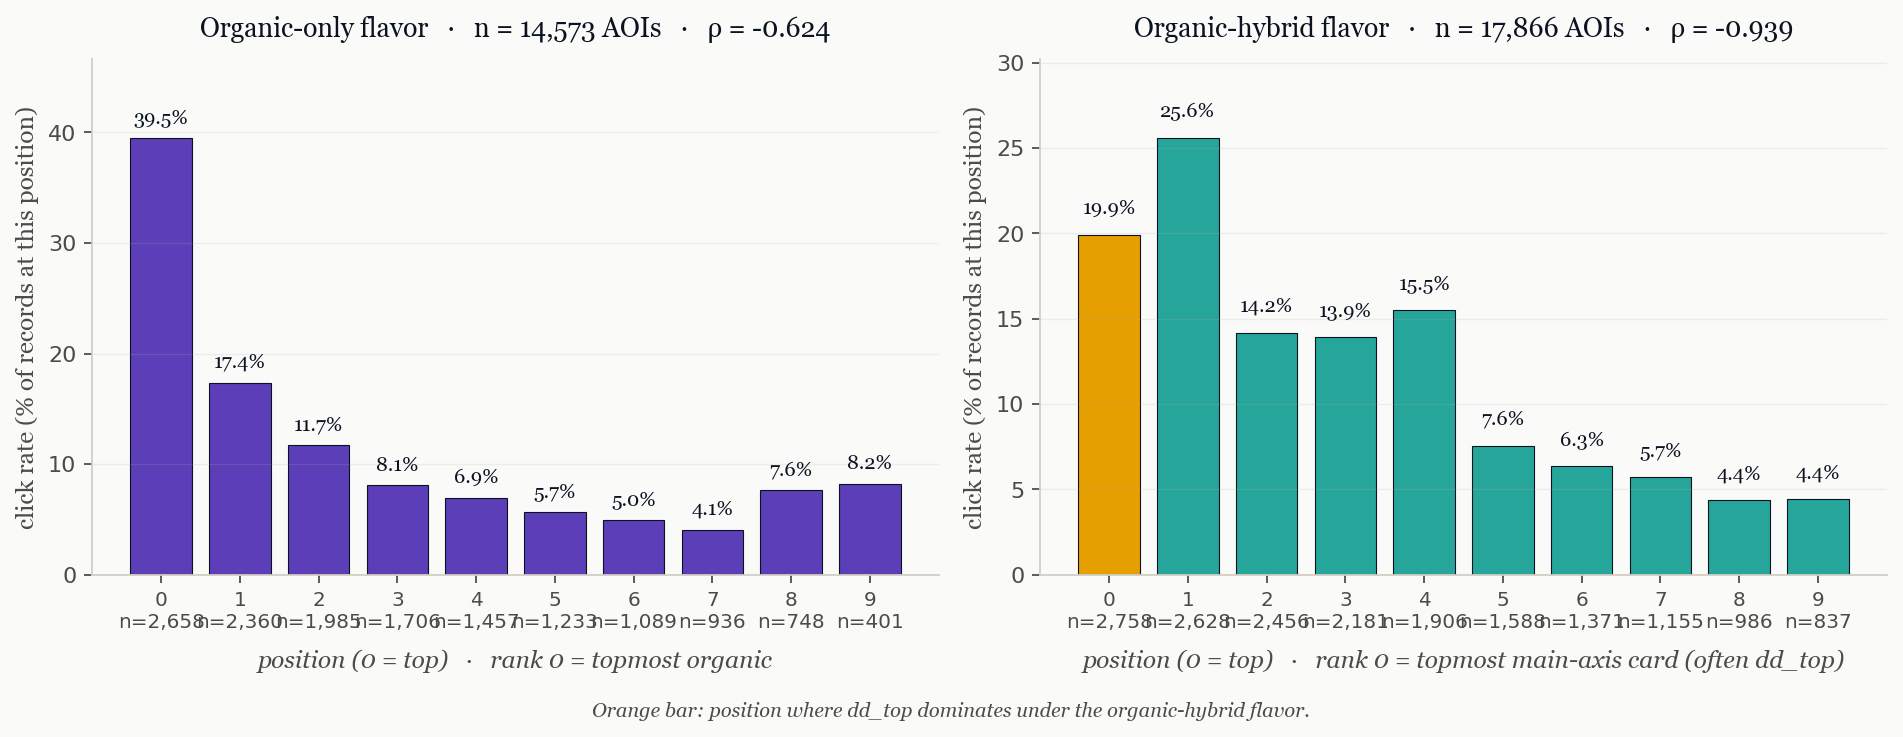
\includegraphics[width=\textwidth]{figs/fig_rank_effects.png}
  \Description[Two bar charts comparing click rate by position under two position-numbering conventions]{Two side-by-side bar charts of click rate by SERP position 0 to 9. The left chart, organic-only positions in purple, shows position 0 at 39.5 percent declining steeply to 4 to 8 percent at positions 7 plus. The right chart, all-main-axis positions in teal, shows position 0 at 19.9 percent (highlighted in orange to mark dd\_top dominance), with the click peak at position 1 at 25.6 percent and gradual decline thereafter.}
  \caption{Click rate by SERP position under two position-numbering conventions, orthogonal to the bbox flavors of \S\ref{sec:pipeline}. Per-bar $n$ is the number of AOIs at each position, and the panel header gives the total over positions 0--9. Click rate at each position is computed within that bar's denominator only. \textbf{Left, organic-only positions} (positions index only organic results; 14,760 AOIs total, 74\,\% of the main-axis population). Position 0 is the topmost organic and the click heavyweight (39.5\,\%). Ranks decline to 4--8\,\% by position 7+ (Spearman $\rho = -0.624$). \textbf{Right, all-main-axis positions} (positions index every main-axis card, including \texttt{dd\_top} ads and widgets; 19,908 AOIs). Position 0 is the topmost main-axis card, often a \texttt{dd\_top} ad (orange bar, 19.9\,\%). The click peak shifts to position 1 (25.6\,\%), where the top organic now sits ($\rho = -0.939$). Consumers should pick the convention that matches their question: ``what does the top organic earn?'' versus ``what does the topmost SERP slot earn?''.}
  \label{fig:rank}
\end{figure*}

\section{Limitations and Public Release}\label{sec:release}

\subsection{Scope and provenance}

\paragraph{Forced-choice task design} AdSERP elicits one click per query within a 1-minute window (extended to 2~minutes after a confirmation prompt) on a single query phrase per trial. The corpus does not sample query refinement, query reformulation, pagination, abandonment, multi-query sessions, or decision arcs longer than the forced-choice envelope. Behavioral statistics in \S\ref{sec:inventory} are properties of constrained-choice SERP evaluation, not of free Google search.

\paragraph{Pre-AI-Overviews snapshot} Data were collected between 2022-12-16 and 2023-03-13 (verified from per-trial entry timestamps), predating Google's AI Overviews / SGE rollout (limited test May 2023, broad deployment May 2024) and Bard's launch (March 21, 2023, three days after collection ended). This is a \emph{feature}: AllSERP is the canonical pre-SGE snapshot of commercial-intent Google SERP behavior, an artifact whose value as a baseline grows over time. Replications on post-May-2024 SERPs need an additional \texttt{ai\_overview} etype, and the AI answer card has substantively different click-fixation dynamics. The four-phase pipeline shape is era-agnostic, and only Phase~B's label set needs to grow.

\paragraph{Phase~D heuristic} The midpoint-split is a heuristic for the boundary between adjacent organic results, not DOM-derived ground truth. Misattribution is bounded by inter-result gap size (typically 5--60~px). We ship both flavors so consumers pick.

\paragraph{Top-ads column subdivision} The current release types every \texttt{dd\_top} card as a single AOI. Multi-column top-ads layouts (2--3 sponsored cards arranged side-by-side above the organic results) are typed as one block rather than subdivided per column. Per-column subdivision is a planned update.

\paragraph{Right-rail coverage} The pipeline tracks shipped \texttt{dd\_right} rectangles for off-axis classification but does not recover right-rail organic-style results. $\sim$1\,\% of trials show a right-rail click that has no shipped rectangle. This is a property of the original release.

\paragraph{Provenance} AdSERP collection followed the original team's approved IRB~\cite{latifzadeh2025adserp}. AllSERP processes only de-identified telemetry and screenshots already released under CC-BY-4.0.

\subsection{Public release}\label{sec:public-release}

\begin{itemize}
  \item \textbf{Code.} \texttt{attentional-foraging} (\url{https://github.com/andyed/attentional-foraging}) and \texttt{approach-retreat} (\url{https://github.com/andyed/approach-retreat}) under MIT license. Single-script entry point at \path{scripts/build_aois.py}.
  \item \textbf{Derived data (CC-BY-4.0).} The release ships two corpus-CSV flavors of per-AOI geometry plus matching per-trial JSONs ($\sim$19~MB across 2,776 trials) and a per-(trial, position) content-feature file with lexical, query-overlap, and semantic-cosine features:
  \begin{itemize}
    \item \path{adserp_aois_by_trial_id_typed_gapfill.csv} --- 9-etype gap-fill flavor (Phase A $\rightarrow$ D). \textbf{Recommended default} and the basis for the inventory in \S\ref{sec:inventory}.
    \item \path{adserp_aois_by_trial_id_organic_hybrid.csv} --- 3-etype taxonomy (\texttt{organic}, \texttt{native\_ad}, \texttt{dd\_top}) with all-main-axis position numbering. Non-ad widgets (PAA, knowledge panels, image packs, top\_places, other widgets) are pooled into \texttt{organic}, so the \texttt{organic} row count (26,590) exceeds \texttt{typed\_gapfill}'s (22,354). Use this flavor for continuous position-rank analyses where the topmost SERP slot is the unit of interest; use \texttt{typed\_gapfill} when per-widget fixation or pupil signals must be disambiguated. Fig.~\ref{fig:rank} (right panel) uses this flavor.
  \end{itemize}
  A third flavor adding per-column subdivision of multi-column \texttt{dd\_top} top-ads is planned. The repo README documents the methodology and a snippet-TTR rank-confound caveat that consumers must partial out before per-position content claims.
  \item \textbf{Replay viewer.} \url{https://andyed.github.io/approach-retreat/replay/} renders typed AOIs on the source SERP screenshots for 147 curated trials.
  \item \textbf{Underlying corpus.} AllSERP requires the AdSERP Zenodo volume (\url{https://zenodo.org/records/15236546}). AdSERP authors release it CC-BY-4.0, and AllSERP does not redistribute screenshots or HTML.
\end{itemize}

\paragraph{Use} The corpus CSV is the join target for downstream click-rate, fixation, and content-feature analyses. Existing AdSERP signal files (cursor approach features, pupil power-ratio, saccade orientation) merge on \texttt{trial\_id} and gain a per-AOI \texttt{etype} column without re-collecting data. The \texttt{attentional-foraging} README ships a minimal Polars worked example (corpus CSV $\rightarrow$ above-fold organic count; cursor-approach features $\rightarrow$ per-position click rate; per-trial JSON $\rightarrow$ typed-AOI inspection).

\subsection{Citation}

AllSERP ships only the typed AOI labels and the extraction pipeline. The shipped AOIs are pixel-anchored to AdSERP screenshots and indexed by AdSERP trial IDs, so any analysis that joins them to gaze, cursor, scroll, or pupil streams requires the AdSERP corpus, and both citations apply. The only standalone use case for AllSERP is applying the pipeline to a different SERP corpus, in which case the AllSERP citation alone suffices.

\begin{verbatim}
@misc{edmonds2026allserp,
  author = {Edmonds, Andy},
  title  = {{AllSERP}: Exhaustive Per-Element
            Enrichment of the Versatile
            {AdSERP} Dataset},
  year   = {2026},
  eprint = {arXiv:XXXX.XXXXX},
  archivePrefix = {arXiv}
}

@inproceedings{latifzadeh2025adserp,
  author    = {Latifzadeh, Kayhan and
               Gwizdka, Jacek and
               Leiva, Luis A.},
  title     = {A Versatile Dataset of Mouse
               and Eye Movements on Search
               Engine Results Pages},
  booktitle = {SIGIR '25},
  year      = {2025},
  pages     = {3412--3421},
  doi       = {10.1145/3726302.3730325}
}
\end{verbatim}

\section{Conclusion}\label{sec:conclusion}

AllSERP is a typed AOI and per-element behavioral enrichment of the AdSERP corpus. The pipeline anchors bbox geometry to the shipped screenshots, types every element via an 8-tier HTML parser, and fills inter-result Y gaps via midpoint-split. The Phase~C ad partition is internally consistent with shipped ground truth across 38,250 classifications. Click attribution under X+Y containment reaches 91.7\,\% of the corpus. The descriptive observations in \S\ref{sec:inventory} surface click-fixation dissociation, regressive return rates, and above-fold geometry at per-element granularity that the prior ad-vs-organic split did not resolve.

The substrate the enrichment unlocks is broader than the four metrics inventoried here. With per-element labels and geometry now joined to the multimodal telemetry the AdSERP team released, several lines of work become tractable on the existing 2,776-trial corpus without re-collecting data. Cursor approach-retreat episode geometry can be computed per AOI rather than per rank, exposing the shape of the decision moment as a function of element type. Pupillometric and LF/HF cognitive-load signals~\cite{duchowski2026rtlfhf,jayawardena2025ripa2} can be conditioned on element type, separating the load profile of an organic-result inspection from a knowledge-panel scan or an ad-card glance. Content-feature analyses can be paired with element-type and behavioral outcomes to ask which content properties co-vary with engagement on which surfaces. Information-foraging theory~\cite{pirolli1999foraging,fu2007snifact} provides a natural theoretical lens here, with query-snippet semantic cosine and query-token overlap as operational proxies for information scent at the per-AOI level.

What ships here is the geometric and typing layer those next steps depend on. The behavioral inventory in \S\ref{sec:inventory} is the descriptive baseline. The analyses it enables are the work the field can now do on a clean pre-AI-Overviews snapshot of commercial-intent SERP behavior, while the four-phase pipeline shape stays era-agnostic for replications on post-rollout SERPs. We are optimistic about the breadth of IR and HCI work the dataset can support.

\section{AI Use Disclosure}\label{sec:aiuse}

This paper was drafted in collaboration with Anthropic's Claude (Opus~4.7). Two automated audit tools kept the draft honest. \mbox{\texttt{science-agent}} (\url{https://github.com/andyed/science-agent}) cross-referenced every citation against the bibliography and lit-notes, verifying that prose paraphrases matched each cited work's actual claims. A second argument-rigor pass flagged ungrounded comparatives, causal language in descriptive prose, and numerical mismatches across sections, tables, and figure captions. The numbers in this paper come from a pipeline disciplined by stable Key-Claim identifiers in the upstream notebooks, which made mid-draft revisions cheap to recompute end-to-end without hand-typing or interpretation drift. Null findings are tracked alongside positive results in the released artifact. All quantitative claims, citations, and methodological decisions were verified by the authors, who take full responsibility for the content.

\begin{acks}
Thanks to Peter Dixon for code review and collaboration on downstream use cases.
\end{acks}

\bibliographystyle{ACM-Reference-Format}
\bibliography{bib/allserp}

\end{document}
